\documentclass[12pt,twoside]{article}
\usepackage[dvipsnames]{xcolor}
\usepackage{tikz,graphicx,amsmath,amsfonts,amscd,amssymb,bm,cite,epsfig,epsf,url}
\usepackage[hang,flushmargin]{footmisc}
\usepackage[colorlinks=true,urlcolor=blue,citecolor=blue]{hyperref}
\usepackage{amsthm,multirow,wasysym,appendix}
\usepackage{array,subcaption} 
% \usepackage[small,bf]{caption}
\usepackage{bbm}
\usepackage{pgfplots}
\usetikzlibrary{spy}
\usepgfplotslibrary{external}
\usepgfplotslibrary{fillbetween}
\usetikzlibrary{arrows,automata}
\usepackage{thmtools}
\usepackage{blkarray} 
\usepackage{textcomp}
\usepackage[left=0.8in,right=1.0in,top=1.0in,bottom=1.0in]{geometry}
\usepackage{pdfpages}

\title{Linear Algebra HW 5}
\author{gjd9961 }
\date{October 2021}

\begin{document}

\maketitle

\section{Problem 5.1}
Give an othonormal basis of $\mathbb{R}^3$ using the Gram-Schmidt algorithm starting from the linearly independent family $(v_1, v_2, v_3)$ where $v_1 = (1, 1, 1)$, $v_2 = (2, 1, 1)$ and $v_3 = (2, 0, 1)$.
\\

Lets begin making an orthonomal set, $x$ out of our linearly independent family, $v$. To start our algorithm, we will need to normalize $v_1$ such that its norm is equal to 1, to make our $x_1$. We can accomplish this with the following: $$x_1 = \frac{v_1}{||v_1||} = (1,1,1) \times (\sqrt{\frac{1}{3}}) = (\sqrt{\frac{1}{3}},\sqrt{\frac{1}{3}},\sqrt{\frac{1}{3}}) \text{ Now }  ||x_1|| = ||\frac{v_1}{||v_1||}|| = \frac{||v_1||}{||v_1||} = 1$$ 
Although we did some operations $v_1$ and $x_1$, $x_1$ is still some linear combinations of $v_1$ still share the same span, and have the same dimension, and are the same subspace, as all we changed was the magnitude of the norm. That is to say 

$$dim(span(v_1)) = 1 = dim(span(x_1)) \text{ and } span(x_1) \subset span(v_1) \text{ therefore } x_1 = v_1$$

Now that $x_1$ has an Euclidean norm of 1, we can begin to make the rest of our orthonormal basis, starting with $x_2$. To compute $x_2$ we will perform the following operaiton:
\begin{equation}
    \begin{split}
        x_2 = x_2 - \langle x_1, v_2\rangle \times x_1 = (2,1,1)  - (4\sqrt{\frac{1}{3}}) \times  (\sqrt{\frac{1}{3}},\sqrt{\frac{1}{3}},\sqrt{\frac{1}{3}}) = (\frac{2}{3},-\frac{1}{3},-\frac{1}{3})
    \end{split}
\end{equation}
Our $x_2$ is now orthogonal to $x_1$, but we need to normalize $x_2$ to ensure our basis is orthonormal
\begin{equation}
    \begin{split}
        x_2 = \frac{x_2}{||x_2||} = (\frac{2}{3},-\frac{1}{3},-\frac{1}{3}) \times \
        \frac{1}{\sqrt{\frac{2}{3}}}   = (\frac{\sqrt{6}}{3},- \frac{\sqrt{6}}{6}, - \frac{\sqrt{6}}{6}) \text{ and } ||x_2|| = ||\frac{x_2}{||x_2||}|| = \frac{||x_2||}{||x_2||} = 1
    \end{split}
\end{equation}

$x_2$ is now normalized to have a Euclidian norm of 1. We can check that $x_1$ and $x_2$ are orthogonal to one another:
$$
    \langle x_1, x_2\rangle = \langle x_2 - \langle x_1,v_2\rangle \times x_1 , x_1 \rangle = \langle x_2, x_1 \rangle - \langle x_1 \times \langle x_1, v_2 \rangle, x_1 \rangle = \langle x_2,x_1 \rangle - \langle x_2,x_1 \rangle \times \langle x_1, x_1 \rangle = 0 
$$
We have confirmed that $x_1 \perp x_2$ by checking that $\langle x_2,x_1 \rangle = 0$, and we made sure to normalize both $x_1,x_2$ so as of right now we have an orthonormal family of vectors. Now for the final piece, we must derive $x_3$ from $v_3$ by doing the following operation:

\begin{equation}
    \begin{split}
    x_3 = v_3 - x_2 \langle x_2, v_3\rangle - x_1 \langle x_1, v_3 \rangle 
    \end{split}
\end{equation}

\begin{equation}
    \begin{split}
         = (2,0,1) - ((\frac{\sqrt{6}}{3},- \frac{\sqrt{6}}{6}, - \frac{\sqrt{6}}{6}) \times \frac{\sqrt{6}}{2})) - ((\frac{2}{3},-\frac{1}{3},-\frac{1}{3}) \times \frac{1}{3} = (0, -\frac{1}{2}, \frac{1}{2})
    \end{split}
\end{equation}
We now have our third orthogonal vector $x_3$, but we need to normalize it:
$$
    x_3 = \frac{x_3}{||x_3||} =  (0, -\frac{1}{2}, \frac{1}{2}) \times  \frac{1}{\frac{1}{\sqrt{2}}} = (0, -\frac{\sqrt{2}}{2}, \frac{\sqrt{2}}{2}) \rightarrow ||x_3|| = \frac{||x_3||}{||x_3||} = 1
$$
Now we have the following orthonormal basis: 
$$\{x_1,x_2,x_3 \} = \begin{pmatrix}
\frac{\sqrt{3}}{3} & \frac{\sqrt{6}}{3} & 0 \\
\frac{\sqrt{3}}{3} & -\frac{\sqrt{6}}{6} & -\frac{\sqrt{2}}{2}\\
\frac{\sqrt{3}}{3} & -\frac{\sqrt{6}}{6} & \frac{\sqrt{2}}{2} \\
\end{pmatrix}$$
Lets ensure that this is an orthonormal basis with the following:\\
$x_3$ is orthogonal to $x_1, x_2$
$$
    \langle x_3,x_2 + x_1 \rangle = \langle x_3, x_2 \rangle + \langle x_3, x_1 \rangle = \langle v_3, x_2 \rangle - \langle x_2, v_3 \rangle \times \langle x_2, x_2 \rangle + \langle v_3, x_1 \rangle - \langle v_3, x_1 \rangle \times \langle x_1, x_1 \rangle = 0
$$
We know that we have normalized all of our basis vectors to Euclidean norm equal to 1, so we have a valid orthonormal basis.\\

Since we have 3 lineraly independent vectors, the span of our new basis is equal to the span of the linearly independent basis we started with. That is to say:
$$
    dim(span(x_1,x_2,x_3))  = 3 = dim(span(v_1,v_2,v_3))
$$
Lastly, we know that $\{x_1,x_2,x_3 \}$ are linearly combinations of $\{v_1, v_2, v_3 \}$ which means:
$$
    span(x_1,x_2,x_3) \subset span(v_1,v_2,v_3)
$$  

By lecture 1, since $dim(span(x_1,x_2,x_3)) = dim(span(v_1,v_2,v_3))$ and $span(x_1,x_2,x_3) \subset span(v_1,v_2,v_3)$ then the family of vectors $x$ is equal to the family of vectors $=v$

\break


\section{Problem 5.2}
Consider $ U = span((\frac 1 2, \frac 1 2, \frac 1 2, \frac 1 2))$ and $V = span((1, 0, 0, 0),(0, 1, 0, 0))$, two subspaces of $\mathbb{R}^4$. \\

a) Compute the canonical matrix $M_U \in \mathbb{R}^{4\times 4}$ of orthogonal projection $P_U(\cdot)$ onto subspace $U$. What is the rank of $M_U$?
\\

We can compute the canonical matrix $M_U \in \mathbb{R}^{4\times 4}$ of the orthogonal projection  $P_U(\cdot)$ onto the subspace $U$ with the matrix projection formula of $UU^T$
$$
    M_U = UU^T = \begin{pmatrix} \frac{1}{2} \\ \frac{1}{2} \\ \frac{1}{2} \\ \frac{1}{2} \end{pmatrix} \times (\frac{1}{2}, \frac{1}{2}, \frac{1}{2}, \frac{1}{2}) = \begin{pmatrix}
        \frac{1}{4} & \frac{1}{4} & \frac{1}{4} & \frac{1}{4} \\
        \frac{1}{4} & \frac{1}{4} & \frac{1}{4} & \frac{1}{4} \\
        \frac{1}{4} & \frac{1}{4} & \frac{1}{4} & \frac{1}{4} \\
        \frac{1}{4} & \frac{1}{4} & \frac{1}{4} & \frac{1}{4} \\
    \end{pmatrix} \text{Row echelon: } \begin{pmatrix} 
        \frac{1}{4} & \frac{1}{4} & \frac{1}{4} & \frac{1}{4} \\
        0 & 0 & 0 & 0\\
        0 & 0 & 0 & 0 \\
        0 & 0 & 0 & 0 \\
        \end{pmatrix} \text{ By doing $R_{2,3,4} - R_1$}
 $$
 
After we calculated the row echelon form, we can see that there is only 1 linearly independent column $(\frac{1}{2},\frac{1}{2},\frac{1}{2},\frac{1}{2})$, and three free variables. Therefore, $Dim(Ker(M_U)) = 3$ and $Rank(M_U) = Dim(Span(M_U)) = 1$
\\

b) Compute the canonical matrix $M_V \in \mathbb{R}^{4\times 4}$ of orthogonal projection $P_V(\cdot)$ onto subspace $V$. What is the rank of $M_V$?
\\

We can calculate the canonimal matrix $M_V \in \mathbb{R}^{4\times 4}$ of orthogonal projection $P_V(\cdot)$ onto subspace $V$ with the same process we used in part 1.
$$
    M_V = VV^T = \begin{pmatrix} 
    1 & 0 \\
    0 & 1 \\
    0 & 0 \\
    0 & 0 
    \end{pmatrix} \times
    \begin{pmatrix}
    1 & 0 & 0 & 0 \\
    0 & 1 & 0 & 0 
    \end{pmatrix} = 
    \begin{pmatrix}
    1 & 0 & 0 & 0\\
    0 & 1 & 0 & 0\\
    0 & 0 & 0 & 0\\
    0 & 0 & 0 & 0
    \end{pmatrix}
$$

We can see clearly that we have 2 linearly independent columns in $M_V$ $(1,0,0,0)$ and $(0,1,0,0)$. That means $Dim(Ker(M_V)) = 2$ and $Rank(M_V) = Dim(Span(M_V)) = 2$ \\

c) Let $x=(1,2,3,4)$ in $\mathbb{R}^4$, compute $y = P_U \circ P_V (x)$ and $z = P_V \circ P_U (x)$. Do we have $y = z$?
\\
Lets compute $y = P_U \circ P_V (x)$ first.
$$
    y = P_U \circ P_V (x) = M_U \circ M_V (x) = \begin{pmatrix}
        \frac{1}{4} & \frac{1}{4} & \frac{1}{4} & \frac{1}{4} \\
        \frac{1}{4} & \frac{1}{4} & \frac{1}{4} & \frac{1}{4} \\
        \frac{1}{4} & \frac{1}{4} & \frac{1}{4} & \frac{1}{4} \\
        \frac{1}{4} & \frac{1}{4} & \frac{1}{4} & \frac{1}{4} \\
    \end{pmatrix} \times    \begin{pmatrix}
    1 & 0 & 0 & 0\\
    0 & 1 & 0 & 0\\
    0 & 0 & 0 & 0\\
    0 & 0 & 0 & 0
    \end{pmatrix} \times \begin{pmatrix}
    1 \\
    2\\
    3\\
    4
    \end{pmatrix} = 
    \begin{pmatrix}
    .75 \\
    .75\\
    .75\\
    .75
    \end{pmatrix}
$$

Now lets compute $z = P_V \circ P_U (x)$

$$
 z = P_V \circ P_U(x) = M_V \circ M_U =  \begin{pmatrix}
    1 & 0 & 0 & 0\\
    0 & 1 & 0 & 0\\
    0 & 0 & 0 & 0\\
    0 & 0 & 0 & 0
    \end{pmatrix} \times 
    \begin{pmatrix}
        \frac{1}{4} & \frac{1}{4} & \frac{1}{4} & \frac{1}{4} \\
        \frac{1}{4} & \frac{1}{4} & \frac{1}{4} & \frac{1}{4} \\
        \frac{1}{4} & \frac{1}{4} & \frac{1}{4} & \frac{1}{4} \\
        \frac{1}{4} & \frac{1}{4} & \frac{1}{4} & \frac{1}{4} \\
    \end{pmatrix} \times 
     \begin{pmatrix}
    1 \\
    2\\
    3\\
    4
    \end{pmatrix} = 
 \begin{pmatrix}
    2.5\\
    2.5\\
    0\\
    0
    \end{pmatrix}
$$

We can clearly see that $y=(.75,.75,.75,.75) \neq z = (2.5,2.5,0,0)$ \\



d) Compute the matrix products $M_U M_V$ and $M_V M_U$. Do $M_U$ and $M_V$ "commute", meaning do we have $M_U M_V = M_V M_U$. Can you give an intuition of why it is the case looking the definitions of $U$ and $V$?
\\

Lets firstly compute $M_U M_V$:
$$
    M_UM_V =  \begin{pmatrix}
        \frac{1}{4} & \frac{1}{4} & \frac{1}{4} & \frac{1}{4} \\
        \frac{1}{4} & \frac{1}{4} & \frac{1}{4} & \frac{1}{4} \\
        \frac{1}{4} & \frac{1}{4} & \frac{1}{4} & \frac{1}{4} \\
        \frac{1}{4} & \frac{1}{4} & \frac{1}{4} & \frac{1}{4} \\
    \end{pmatrix} \times    \begin{pmatrix}
    1 & 0 & 0 & 0\\
    0 & 1 & 0 & 0\\
    0 & 0 & 0 & 0\\
    0 & 0 & 0 & 0 
    \end{pmatrix} = 
    \begin{pmatrix}
    .25 & .25 & 0 & 0\\
    .25 & .25 & 0 & 0\\
    .25 & .25 & 0 & 0\\
    .25 & .25 & 0 & 0\\
    \end{pmatrix}
$$

Lets now compute $M_V M_U$

$$
    M_V M_U = 
    \begin{pmatrix}
    1 & 0 & 0 & 0\\
    0 & 1 & 0 & 0\\
    0 & 0 & 0 & 0\\
    0 & 0 & 0 & 0 
    \end{pmatrix} \times
    \begin{pmatrix}
        \frac{1}{4} & \frac{1}{4} & \frac{1}{4} & \frac{1}{4} \\
        \frac{1}{4} & \frac{1}{4} & \frac{1}{4} & \frac{1}{4} \\
        \frac{1}{4} & \frac{1}{4} & \frac{1}{4} & \frac{1}{4} \\
        \frac{1}{4} & \frac{1}{4} & \frac{1}{4} & \frac{1}{4} \\
    \end{pmatrix}
    =
    \begin{pmatrix}
    .25 & .25 & .25 & .25\\
    .25 & .25 & .25 & .25\\
    0 & 0 & 0 & 0\\
    0 & 0 & 0 & 0 
    \end{pmatrix}
$$
We can see that the two matrix compositions do not commute, that is to say that $M_VM_U \neq M_UM_V$ This is because the two sub-spaces we are projecting into have no span that overlaps, and furthermore, have different dimensions. Therefore, the order in which we project matters. If we first project using $P_V$ then project into $P_U$, we are essentially projecting a vector first into a two dimensional subspace, then a one dimensional line. If we project a vector into $P_U$ then project it into $P_V$ we are firstly projecting a vector onto a one dimensional subspace (a line), and then onto a two dimensional subspace (a hyper-plane). In each sequence of projections, we lose different amounts of information at different times due to the dimension of $M_U$ and $M_V$ and also we end up in different sub-spaces. Therefore, it makes intuitive sense that the matrices do not commute. \\

e) Considering now $ U' = span \left((\frac{1}{\sqrt{2}}, \frac{1}{ \sqrt{2}}, 0, 0)\right)$. Compute $M_{U'}$. Do we have $M_{U'}M_V = M_{V}M_{U'}$? Can you give an intuition why?\\

Firstly, lets compute $M_U'$
$$
    M_{U'} = U' U^T' = \begin{pmatrix}
    \frac{1}{\sqrt{2}}\\
        \frac{1}{\sqrt{2}}\\
        0\\
        0
    \end{pmatrix} \times (\frac{1}{\sqrt{2}},\frac{1}{\sqrt{2}},0,0) = 
    \begin{pmatrix}
    \frac{1}{2} &     \frac{1}{2} & 0 & 0 \\
        \frac{1}{2} &     \frac{1}{2} & 0 & 0 \\
        0 & 0 & 0 & 0 \\
        0 & 0 & 0 & 0
    \end{pmatrix}
$$
Now lets compute $M_U' M_V$
$$
    M_U' M_V =    \begin{pmatrix}
    \frac{1}{2} &     \frac{1}{2} & 0 & 0 \\
        \frac{1}{2} &     \frac{1}{2} & 0 & 0 \\
        0 & 0 & 0 & 0 \\
        0 & 0 & 0 & 0
    \end{pmatrix} \times \begin{pmatrix}
    1 & 0 & 0 & 0\\
    0 & 1 & 0 & 0\\
    0 & 0 & 0 & 0\\
    0 & 0 & 0 & 0 
    \end{pmatrix}
    = \begin{pmatrix}
    \frac{1}{2} &     \frac{1}{2} & 0 & 0 \\
        \frac{1}{2} &     \frac{1}{2} & 0 & 0 \\
        0 & 0 & 0 & 0 \\
        0 & 0 & 0 & 0 \end{pmatrix}
$$  

Now lets compute $M_V M_U'$:
$$
M_V M_U' = \begin{pmatrix}
    1 & 0 & 0 & 0\\
    0 & 1 & 0 & 0\\
    0 & 0 & 0 & 0\\
    0 & 0 & 0 & 0 
    \end{pmatrix} \times \begin{pmatrix}
    \frac{1}{2} &     \frac{1}{2} & 0 & 0 \\
        \frac{1}{2} &     \frac{1}{2} & 0 & 0 \\
        0 & 0 & 0 & 0 \\
        0 & 0 & 0 & 0
    \end{pmatrix} = 
    \begin{pmatrix}
    \frac{1}{2} &     \frac{1}{2} & 0 & 0 \\
        \frac{1}{2} &     \frac{1}{2} & 0 & 0 \\
        0 & 0 & 0 & 0 \\
        0 & 0 & 0 & 0
    \end{pmatrix}
$$
Now we do have $M_U' M_V = M_V M_U'$. In this case, the matrix multiplication is commutative because the Span of $M_U'$ is a subset of the Span of $M_V$. Therefore, when we project a vector into the subspace spanned by $M_U'$ with the transformation $P_{U'}(x)$, we are also projecting the vector into the span of $M_V$ as well. If we try to project the same vector we projected into $M_U'$ into $M_V$ using $P_V(x)$, because we are already in the subspace, the projection of the vector will just be the vector itself, and we will essentially be scaling the vector by 1.  

\section{Problem 5.3}
Consider $L$ a linear transformation from $\mathbb{R}^n$ to $\mathbb{R}^n$ and denote by $\tilde L \in \mathbb{R}^{n \times n}$ its canonical matrix. Let $(u_1, \cdot, u_n)$ be any orthonormal basis of $\mathbb{R}^n$ and 
    $$ U = \begin{pmatrix}
        | & & | \\
        u_1 & \cdots & u_n\\
        | & & |
    \end{pmatrix}\in \mathbb{R}^{n \times n}$$.

Show that $\tilde L ' = U^\top \tilde L U$ computes the transformation of vectors in $\mathbb{R}^n$ using coordinates in the basis $(u_1, \cdots, u_n)$.\\

Our expression $\tilde L ' = U^\top \tilde L U$ performs the following transformation: firstly, it takes in a vector with coordinates in the basis $U$, (let's call these coordinates $x'$), which are then transformed into coordinates into the standard basis (lets call these coordinates $x$). Then, the transformation $L$ is applied to the coordinates with the standard basis, producing a vector, (lets call it $y$). Lastly, the vector $y$ is  converted into coordinates the basis $U$, by transforming the vector $y$ by the $U^T$ matrix to produce $y'$. To illustrate this transformation, consider the following. \\

Let $U$ be any orthonormal basis of $\mathbb{R}^n$ and let $x'= U^T x$, and $y' = U^T y$ with $x,y$ being two vectors written in the standard canonical basis of $\mathbb{R}^n$, and $x',y'$ are the vectors $x,y$ with their coordinates expressed in the basis $U$ and  $\{x,y,x',y'\} \in \mathbb{R}^n$

\begin{equation}
    \begin{split}
        \tilde L ' x' = U^T \tilde L U U^T x \text{ We begin by transforming a vector with coordinates in U basis}
    \end{split}
\end{equation}

\begin{equation}
    \begin{split}
        \tilde  U^T \tilde L U U^T x = U^T \tilde L x \text{ The coordinates get converted into the standard basis}
    \end{split}
\end{equation}
\begin{equation}
    \begin{split}
        \tilde  U^T \tilde L x = U^T y \text{ The transformation L is applied to $x$ to produce $y$}
    \end{split}
\end{equation}
\begin{equation}
    \begin{split}
        \tilde  U^T y  = y' \text{ The vector $y$ has its coordinates converted to the basis $U$ }
    \end{split}
\end{equation}
Therefore the transformation $\tilde L ' = U^\top \tilde L U$ computes the transformation of vectors in $\mathbb{R}^n$ using coordinates in the basis $(u_1, \cdots, u_n)$

Alternatively, we can show this the other way around, a little bit more concisely. Lets use the same values of $x,y,x',y',U, \tilde{L}'$
\begin{equation}
\begin{split}
    \tilde{L}'x' = y'
\end{split}\\
\begin{split}
    \tilde{L}'x' = U^Ty
\end{split}\\
\begin{split}
    \tilde{L}'x' = U^T\tilde{L}x
\end{split}\\
\begin{split}
    \tilde{L}'x' = U^T\tilde{L}Ux'
\end{split}\\
\begin{split}
    \tilde{L}'x' = \tilde{L}'x'
\end{split}
\end{equation}
We see this works both ways, and that the transfromation  $\tilde L ' = U^\top \tilde L U$ computes the transformation of vectors in $\mathbb{R}^n$ using coordinates in the basis $(u_1, \cdots, u_n)$.\\

\section{Problem 5.4}
In this problem, we will see how to compress, by using a particular orthonormal basis called a ``discrete cosine basis''.
\\

All the questions are in the jupyter notebook \texttt{DCT.ipynb} and have to be answered directly in the notebook. (Submit only a pdf export of your notebook: Print $\to$ Save as pdf)
\\

You have to use \texttt{Python} and its library \texttt{numpy}. A useful command:
\texttt{ A @ B }: performs the matrix product of the matrix \texttt{A} with the matrix \texttt{B}.

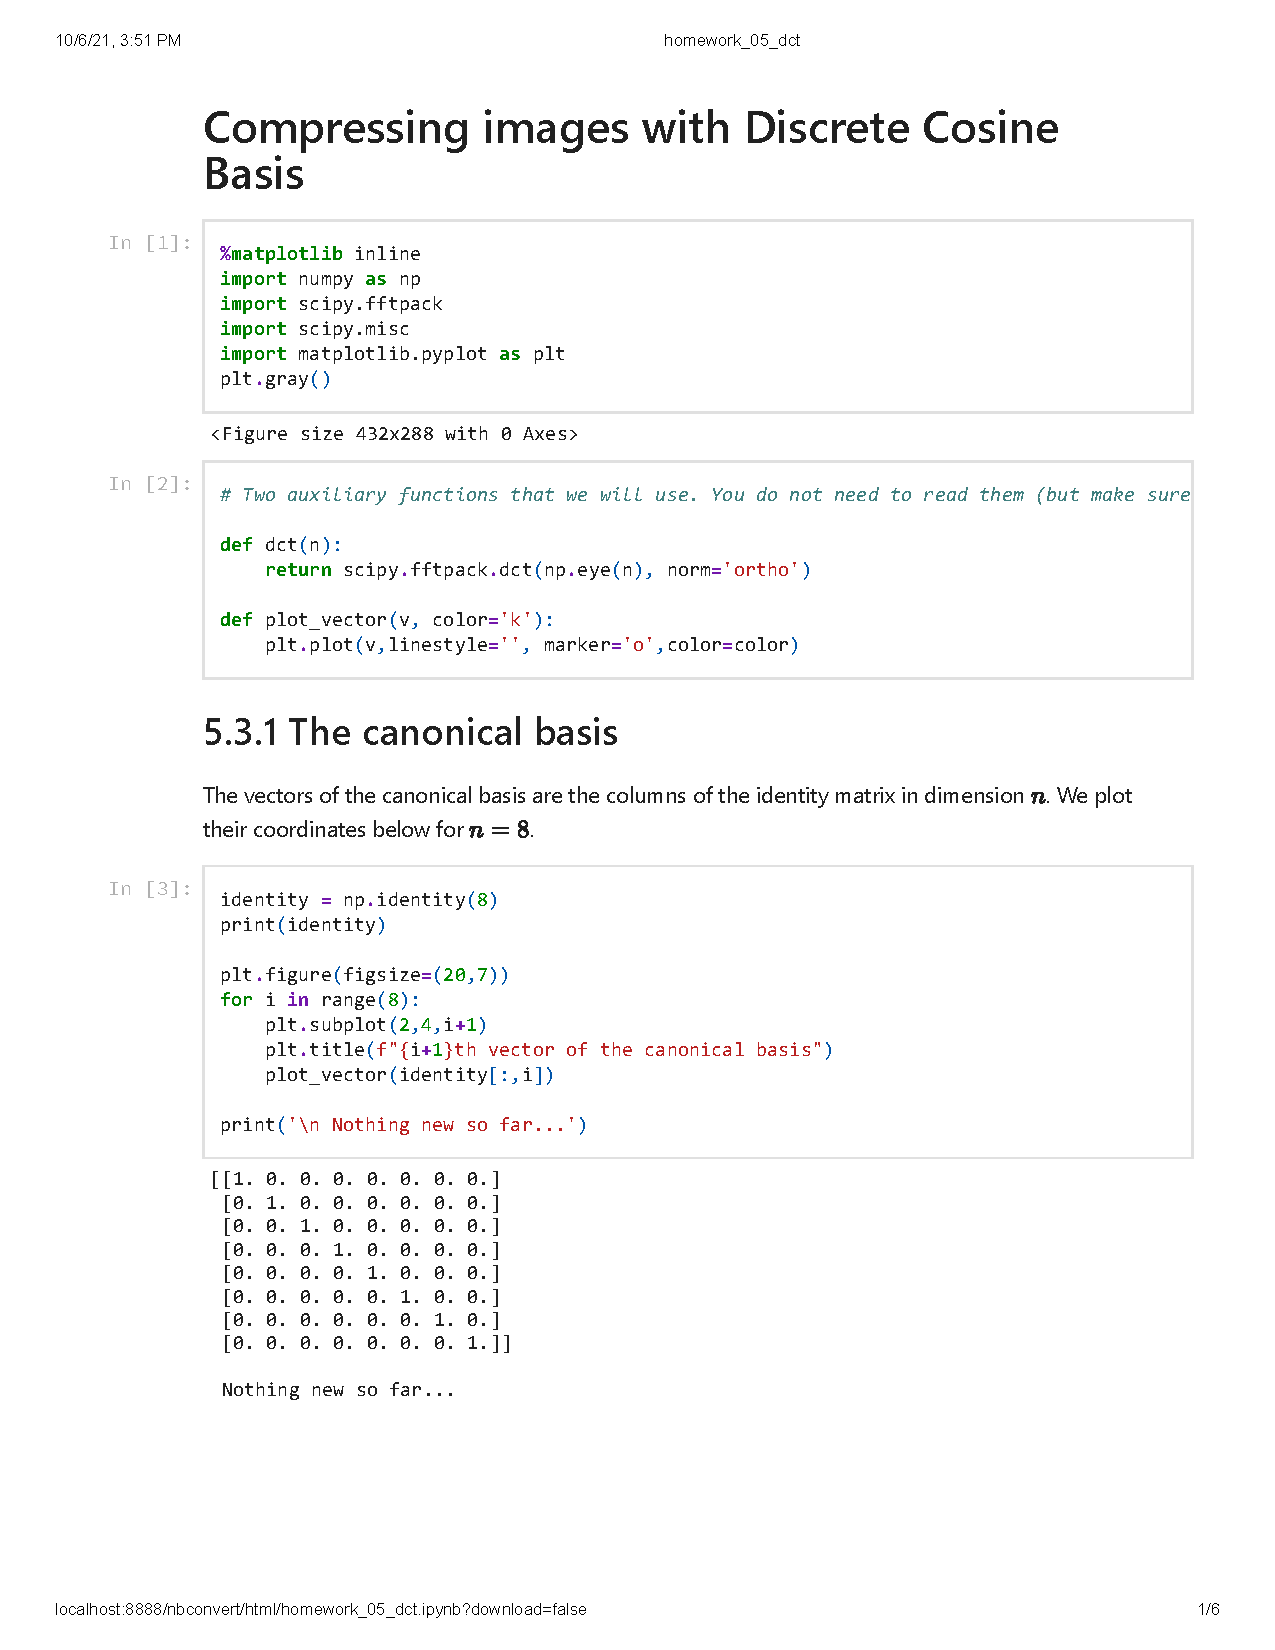
\includepdf[pages=-]{homework_05_dct_giulio_duregon.pdf}

\section{Problem 5.5}
Let $S$ be a subspace of $\mathbb{R}^n$. We define the orthogonal complement of $S$ by
	$$
	S^{\perp} \defeq 
	\big\{ x \in \R^n \, \big| \, x \perp S \big\} = 
	\big\{ x \in \R^n \, \big| \, \forall y \in S, \, \langle x,y \rangle = 0 \big\}.
	$$
a) Show that $S^{\perp}$ is a subspace of $\R^n$.
\\

b)Show that $\dim(S^{\perp}) = n - \dim(S)$. 
\\
c) Show that for any $u \in \R^n$, we can find $x \in S$ and $y \in S^{\perp}$ such that $u = x + y$.





\end{document}


